\chapter{Aufgabe zur komplexen PBZ}

\begin{circuitikz}
  
\end{circuitikz}

\begin{minipage}{0.5\textwidth}
Schaltplan
\end{minipage}
\begin{minipage}{0.5\textwidth}
\begin{itemize}
  \item $S$ ist ein idealer Umschalter, der bei $t=t_1$
    von der unteren in die obere Stellung wechselt
    und bei $t=t_2$ wieder zurückspringt
  \item $v(t)$ ist gegeben durch\\
    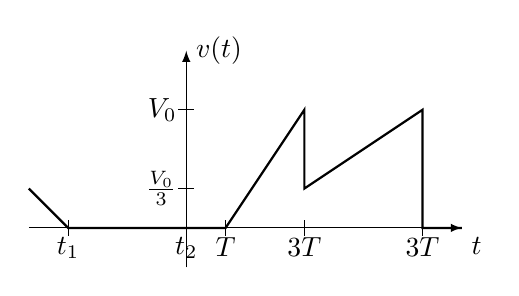
\begin{tikzpicture}[>=latex,scale=0.5]
      \draw[->] (-4,0) -- (7,0) node[below right] {$t$};
      \draw[->] (0,-1) -- (0,4.5) node[right] {$v(t)$};
      %
      \draw[thick] (-4,1)
        -- (-3,0)
        -- (1,0)
        -- (3,3)
        -- (3,1)
        -- (6,3)
        -- (6,0)
        -- (7,0);
      %
      \draw (-3,-0.2) -- + (0,0.4) node[below=1mm] {$t_1$};
      \draw (0,-0.2) -- + (0,0.4) node[below=1mm] {$t_2$};
      \draw (1,-0.2) -- + (0,0.4) node[below=1mm] {$T$};
      \draw (3,-0.2) -- + (0,0.4) node[below=1mm] {$3T$};
      \draw (6,-0.2) -- + (0,0.4) node[below=1mm] {$3T$};
      \draw (-0.2,1) -- + (0.4,0) node[left=1mm] {$\frac{V_0}{3}$};
      \draw (-0.2,3) -- + (0.4,0) node[left=1mm] {$V_0$};
    \end{tikzpicture}
  \item $R_1$, $C_1$, $L_1$, $L_2 > 0$ linear, zeitinvariant,
    $v(t)$ ideale, ungest. SPQ
\end{itemize}
\end{minipage}

Weitere Hinweise:
\begin{enumerate}
  \item $-t_1 >> RC+\frac{L_2}{R} > 0$
  \item Das NWM existiert für alle Zeiten und es gilt $e(t) = v(t)$,
    $a(t) = u_C(t)$ für alle Zeiten
  \item $\frac{L_1}{R} = \frac{43}{104}T$,
    $\frac{L_2}{R} = \frac{43}{111}T$,
    $CL_1 = \frac{1}{43}T^2$
  \item Für $t>0$ ist $\cn A_1 = -\frac{3}{T}<0$ eine nat. Freq.
\end{enumerate}

\textbf{Aufgabe:} Berechnen Sie $u_C(t)$ für \underline{alle} Zeiten.

Lösung zur Aufgabe mit komplexer PBZ

\begin{itemize}
  \item
    Die Anfangswerte sind weder für $t=t_{1,+,-}$ noch für
    $t=t_{2,+,-}$ gegeben\\
    $\Rightarrow$ Betrachte das NWM für $t<t_1$!
  \item
    Für $t<t_1$ und $t>t_2$ ist die Struktur der NWM identisch, dort gilt
    \begin{align*}
      \cn H(\cn s)
        &= \frac{\cn U(\cn s}{\cn V(\cn s)}
         = \frac{%
            R\parallel\left(\frac{1}{\cn sC}+\cn sL_1\right)%
          }{%
            R\parallel\left(\frac{1}{\cn sC}+\cn sL_2\right)
          }
          \cdot\frac{%
            \frac{1}{\cn sC}
          }{%
            \frac{1}{\cn sC}+\cn sL_1
          }\\
        &= -\frac{%
            R\cdot\cancel{\left(\frac{1}{\cn sC}+\cn sL_1\right)}
          }{%
            R\cdot\left(\frac{1}{\cn sC}+\cn sL_1\right)
            +\cn sL_2\left(\cn sL_1+R+\frac{1}{\cn sC}\right)
          }
          \cdot\frac{%
            \frac{1}{\cn sC}
          }{%
            \cancel{\frac{1}{\cn sC}+\cn sL_1}
          }\\
        &= -\frac{%
          R
          }{%
            R\left(\cn s^2CL_1+1\right)+\cn sL_2\left(\cn s^2L_1C+\cn sRC+1\right)
          }\\
        &= -\frac{%
          R
          }{%
            \cn s^3CL_1L_2+\cn s^2RC(L_1+L_2)+\cn sL_2+R
          }\\
        &= -\frac{R}{CL_1L_2}\cdot
          \frac{1}{%
            \cn s^3+\cn s^2\cdot\left(\frac{R}{L_1}+\frac{R}{L_2}\right)
            +\cn s\cdot \frac{1}{CL_1}+\frac{R}{CL_1L_2}
          }\\
        &= \frac{111\cdot \cancel{45}}{\cancel{45}\cdot T^2\cdot T}
          \cdot\frac{1}{%
            \cn s^3+\cn s^2\cdot\frac{\cancel{215}}{\cancel{43}T}+\cn s\cdot\frac{43}{T^2}
            +\frac{111\cdot 43}{43\cdot T^2\cdot T}
          }\\
        &\!\!\!\!\underset{x:=\cn sT}{=} 111\cdot\frac{1}{%
            x^3+5x^2+43x+111
          } = \frac{\cn P(x)}{\cn Q(x)}\\
    \end{align*}

\item $\cn P(s)$, $\cn Q(s)$ sind sicher teilerfremd; außerdem gilt für $t<t_1$
  $t>t_2$: $n_A=3$ ($u_c(t)$, $i_{L_1}(t)$, $i_{L_2}(t)$)\\
  $\Rightarrow$ $3=n_A\geq n\geq \grad(\cn Q(\cn s))=3\quad\Rightarrow\quad n=n_A=3$,
  $\cn Q(\cn s)$ liefert alle nat. Freq, das NWM besitzt keine inkonsitenten AW
  für $t=?$

\item Zeige: Alle nat. Freq haben einen neg. Realteil! Nach Aufgabe:
  $\cn s=-\frac{3}{T} \Rightarrow x_1 = -3$\\
  Mit Horner-Schema geht die Poly-Div schnell:\\
  \[\begin{tabular}{rrrr}
    $1$ & $5$ & $43$ & $111$\\
    \fbox{$-3$} & $-3$ & $-6$ & $-111$\\
    \midrule
    $1$ & $2$ & $37$ & \underline{\underline{$0$}}
  \end{tabular}\]

  $\Rightarrow$ $\cn Q'(x) = (x+3)\cdot (x^2+2x+37) = (x+3)\cdot ((x+1)^2 + 6^2)$
  mit den NSTen von $\cn Q(s)$:
  $\cn s_1 = -\frac{3}{T}$, $s_{2,3}=-\frac{2}{T}\pm j\frac{6}{T}$\\
  $\Rightarrow$ Alle nat. Freq. haben für $t<t_1$, $t>t_2$ einen neg. Realteil,
  das NWM ist dor asympt. stabil!

\item Für $t<t_1$ ist $v(t)=V_0/3$ eine DC-Quelle; das asymptot. stabile NWM
  ex. für alle Zeiten und befindet sich deshalb für $t<t_1$ im EZ;
  sogar im DC-EZ, weil für $t<t_1$ $v(t)$ eine DC-Quelle ist!

  Berechne $u_v(t)$ für $t<t_1$ per DC-ESB, ebenso alle AW für $t=t_1^-$:
  $u_c(t) = -\frac{V_0}{3}=u_c(t_1^-)$, $i_{L_1} = 0$, $i_{L_2} = -\frac{-V_0}{3R}$

\item Beweise Stabilität für $t_1 < t < t_2$; dort ist $v(t)=0$, führe die
  Zeitverschiebung $\tilde t:= t-t_1$ ein!
  \begin{align*}
    \cn H_1(\cn s) &:= \frac{\tilde{\cn U}_{C_1}(\cn s)}{C\cdot u_v(t_1^-)}
    = \frac{1}{\cn sC}\parallel R
    = \frac{R}{\cn sRC+1} = \frac{\cn P_1(\cn s)}{\cn Q_1(\cn s)} \text{ teilerfremd, }\\
    &\cn Q_1(\cn s)\stackrel{!}{=}0
    \Rightarrow \cn s=-\frac{1}{RC}<0\\
    \cn H_2(\cn s) &:= \frac{\tilde{\cn I}_{L_2}(\cn s)}{L_2\cdot i_{L_2}(t_1^-)}
    = \frac{1}{\cn sL_2+R}
    = \frac{\cn P_2(\cn s)}{\cn Q_2(\cn s)} \text{ teilerfremd, }\\
    &\cn Q_2(\cn s)\stackrel{!}{=}0
    \Rightarrow \cn s=-\frac{R}{L_2}<0
  \end{align*}
  Wegen $\frac{R}{L_2}=\frac{111}{43T} \neq \frac{43^2}{104T} = \frac{1}{RC}$
  sind $\cn Q_1(\cn s)$, $\cn Q_2(\cn s)$ teilerfremd.
  Es ist immer noch $n_A=3$, aber $n_R=1$ ($i_{L_1}(t) = 0$)\\
  $\Rightarrow$ $2=n_A-n_R\geq n \geq \grad(\cn Q_1(\cn s))+\grad(\cn Q_2(\cn s))=2$;
  $\cn Q_1(\cn s)$, $\cn Q_2(\cn s)$ liefern alle nat. Freq.
  Sie haben alle einen negativen Reatlteil (s.o.)
  $\Rightarrow$ Das NWM ist für $t_1<t<t_2$ asymptotisch stabil!
\end{itemize}
